% Options for packages loaded elsewhere
\PassOptionsToPackage{unicode}{hyperref}
\PassOptionsToPackage{hyphens}{url}
%
\documentclass[
]{article}
\usepackage{amsmath,amssymb}
\usepackage{iftex}
\usepackage{CTEX}
\ifPDFTeX
  \usepackage[T1]{fontenc}
  \usepackage[utf8]{inputenc}
  \usepackage{textcomp} % provide euro and other symbols
\else % if luatex or xetex
  \usepackage{unicode-math} % this also loads fontspec
  \defaultfontfeatures{Scale=MatchLowercase}
  \defaultfontfeatures[\rmfamily]{Ligatures=TeX,Scale=1}
\fi
\usepackage{lmodern}
\ifPDFTeX\else
  % xetex/luatex font selection
\fi
% Use upquote if available, for straight quotes in verbatim environments
\IfFileExists{upquote.sty}{\usepackage{upquote}}{}
\IfFileExists{microtype.sty}{% use microtype if available
  \usepackage[]{microtype}
  \UseMicrotypeSet[protrusion]{basicmath} % disable protrusion for tt fonts
}{}
\makeatletter
\@ifundefined{KOMAClassName}{% if non-KOMA class
  \IfFileExists{parskip.sty}{%
    \usepackage{parskip}
  }{% else
    \setlength{\parindent}{0pt}
    \setlength{\parskip}{6pt plus 2pt minus 1pt}}
}{% if KOMA class
  \KOMAoptions{parskip=half}}
\makeatother
\usepackage{xcolor}
\usepackage[margin=1in]{geometry}
\usepackage{color}
\usepackage{fancyvrb}
\newcommand{\VerbBar}{|}
\newcommand{\VERB}{\Verb[commandchars=\\\{\}]}
\DefineVerbatimEnvironment{Highlighting}{Verbatim}{commandchars=\\\{\}}
% Add ',fontsize=\small' for more characters per line
\usepackage{framed}
\definecolor{shadecolor}{RGB}{248,248,248}
\newenvironment{Shaded}{\begin{snugshade}}{\end{snugshade}}
\newcommand{\AlertTok}[1]{\textcolor[rgb]{0.94,0.16,0.16}{#1}}
\newcommand{\AnnotationTok}[1]{\textcolor[rgb]{0.56,0.35,0.01}{\textbf{\textit{#1}}}}
\newcommand{\AttributeTok}[1]{\textcolor[rgb]{0.13,0.29,0.53}{#1}}
\newcommand{\BaseNTok}[1]{\textcolor[rgb]{0.00,0.00,0.81}{#1}}
\newcommand{\BuiltInTok}[1]{#1}
\newcommand{\CharTok}[1]{\textcolor[rgb]{0.31,0.60,0.02}{#1}}
\newcommand{\CommentTok}[1]{\textcolor[rgb]{0.56,0.35,0.01}{\textit{#1}}}
\newcommand{\CommentVarTok}[1]{\textcolor[rgb]{0.56,0.35,0.01}{\textbf{\textit{#1}}}}
\newcommand{\ConstantTok}[1]{\textcolor[rgb]{0.56,0.35,0.01}{#1}}
\newcommand{\ControlFlowTok}[1]{\textcolor[rgb]{0.13,0.29,0.53}{\textbf{#1}}}
\newcommand{\DataTypeTok}[1]{\textcolor[rgb]{0.13,0.29,0.53}{#1}}
\newcommand{\DecValTok}[1]{\textcolor[rgb]{0.00,0.00,0.81}{#1}}
\newcommand{\DocumentationTok}[1]{\textcolor[rgb]{0.56,0.35,0.01}{\textbf{\textit{#1}}}}
\newcommand{\ErrorTok}[1]{\textcolor[rgb]{0.64,0.00,0.00}{\textbf{#1}}}
\newcommand{\ExtensionTok}[1]{#1}
\newcommand{\FloatTok}[1]{\textcolor[rgb]{0.00,0.00,0.81}{#1}}
\newcommand{\FunctionTok}[1]{\textcolor[rgb]{0.13,0.29,0.53}{\textbf{#1}}}
\newcommand{\ImportTok}[1]{#1}
\newcommand{\InformationTok}[1]{\textcolor[rgb]{0.56,0.35,0.01}{\textbf{\textit{#1}}}}
\newcommand{\KeywordTok}[1]{\textcolor[rgb]{0.13,0.29,0.53}{\textbf{#1}}}
\newcommand{\NormalTok}[1]{#1}
\newcommand{\OperatorTok}[1]{\textcolor[rgb]{0.81,0.36,0.00}{\textbf{#1}}}
\newcommand{\OtherTok}[1]{\textcolor[rgb]{0.56,0.35,0.01}{#1}}
\newcommand{\PreprocessorTok}[1]{\textcolor[rgb]{0.56,0.35,0.01}{\textit{#1}}}
\newcommand{\RegionMarkerTok}[1]{#1}
\newcommand{\SpecialCharTok}[1]{\textcolor[rgb]{0.81,0.36,0.00}{\textbf{#1}}}
\newcommand{\SpecialStringTok}[1]{\textcolor[rgb]{0.31,0.60,0.02}{#1}}
\newcommand{\StringTok}[1]{\textcolor[rgb]{0.31,0.60,0.02}{#1}}
\newcommand{\VariableTok}[1]{\textcolor[rgb]{0.00,0.00,0.00}{#1}}
\newcommand{\VerbatimStringTok}[1]{\textcolor[rgb]{0.31,0.60,0.02}{#1}}
\newcommand{\WarningTok}[1]{\textcolor[rgb]{0.56,0.35,0.01}{\textbf{\textit{#1}}}}
\usepackage{graphicx}
\makeatletter
\def\maxwidth{\ifdim\Gin@nat@width>\linewidth\linewidth\else\Gin@nat@width\fi}
\def\maxheight{\ifdim\Gin@nat@height>\textheight\textheight\else\Gin@nat@height\fi}
\makeatother
% Scale images if necessary, so that they will not overflow the page
% margins by default, and it is still possible to overwrite the defaults
% using explicit options in \includegraphics[width, height, ...]{}
\setkeys{Gin}{width=\maxwidth,height=\maxheight,keepaspectratio}
% Set default figure placement to htbp
\makeatletter
\def\fps@figure{htbp}
\makeatother
\setlength{\emergencystretch}{3em} % prevent overfull lines
\providecommand{\tightlist}{%
  \setlength{\itemsep}{0pt}\setlength{\parskip}{0pt}}
\setcounter{secnumdepth}{-\maxdimen} % remove section numbering
\ifLuaTeX
  \usepackage{selnolig}  % disable illegal ligatures
\fi
\usepackage{bookmark}
\IfFileExists{xurl.sty}{\usepackage{xurl}}{} % add URL line breaks if available
\urlstyle{same}
\hypersetup{
  pdftitle={地理建模实验2 实验报告},
  pdfauthor={42109232 \quad 吕文博 \quad 地信2101班},
  hidelinks,
  pdfcreator={LaTeX via pandoc}}

\title{地理建模实验2 实验报告}
\author{42109232 \quad 吕文博 \quad 地信2101班}
\date{2024-05-13}

\begin{document}
\maketitle

\subsection{\texorpdfstring{\texttt{Pearson}相关系数计算和散点图绘制}{Pearson相关系数计算和散点图绘制}}\label{pearsonux76f8ux5173ux7cfbux6570ux8ba1ux7b97ux548cux6563ux70b9ux56feux7ed8ux5236}

\begin{Shaded}
\begin{Highlighting}[]
\NormalTok{df\_pearson }\OtherTok{=}\NormalTok{ readxl}\SpecialCharTok{::}\FunctionTok{read\_xls}\NormalTok{(}\StringTok{\textquotesingle{}../data/exp2/2.xls\textquotesingle{}}\NormalTok{,}\AttributeTok{sheet =} \StringTok{\textquotesingle{}Pearson\textquotesingle{}}\NormalTok{)}
\FunctionTok{summary}\NormalTok{(df\_pearson)}
\end{Highlighting}
\end{Shaded}

\begin{verbatim}
##      人名                数学            化学      
##  Length:18          Min.   :50.00   Min.   :60.00  
##  Class :character   1st Qu.:79.25   1st Qu.:81.00  
##  Mode  :character   Median :87.00   Median :88.00  
##                     Mean   :83.56   Mean   :86.61  
##                     3rd Qu.:89.75   3rd Qu.:96.00  
##                     Max.   :99.00   Max.   :99.00
\end{verbatim}

\begin{Shaded}
\begin{Highlighting}[]
\FunctionTok{cor.test}\NormalTok{(df\_pearson}\SpecialCharTok{$}\StringTok{\textasciigrave{}}\AttributeTok{数学}\StringTok{\textasciigrave{}}\NormalTok{,}
\NormalTok{         df\_pearson}\SpecialCharTok{$}\StringTok{\textasciigrave{}}\AttributeTok{化学}\StringTok{\textasciigrave{}}\NormalTok{,}
         \AttributeTok{method =} \StringTok{"pearson"}\NormalTok{)}
\end{Highlighting}
\end{Shaded}

\begin{verbatim}
## 
##  Pearson's product-moment correlation
## 
## data:  df_pearson$数学 and df_pearson$化学
## t = 4.4281, df = 16, p-value = 0.0004219
## alternative hypothesis: true correlation is not equal to 0
## 95 percent confidence interval:
##  0.4210747 0.8978697
## sample estimates:
##       cor 
## 0.7420644
\end{verbatim}

\emph{数学和化学的\texttt{pearson}相关系数为\textbf{0.7420644},P值为\textbf{0.0004219},两者在0.01显著性水平下相关性显著}

\begin{Shaded}
\begin{Highlighting}[]
\FunctionTok{library}\NormalTok{(ggplot2)}

\FunctionTok{ggplot}\NormalTok{() }\SpecialCharTok{+}
  \FunctionTok{geom\_point}\NormalTok{(}\AttributeTok{data =}\NormalTok{ df\_pearson,}
             \FunctionTok{aes}\NormalTok{(}\AttributeTok{x =}\NormalTok{ 数学,}
                 \AttributeTok{y =}\NormalTok{ 化学)) }\SpecialCharTok{+}
  \FunctionTok{coord\_fixed}\NormalTok{() }\SpecialCharTok{+}
  \FunctionTok{theme\_classic}\NormalTok{()}
\end{Highlighting}
\end{Shaded}

\begin{center}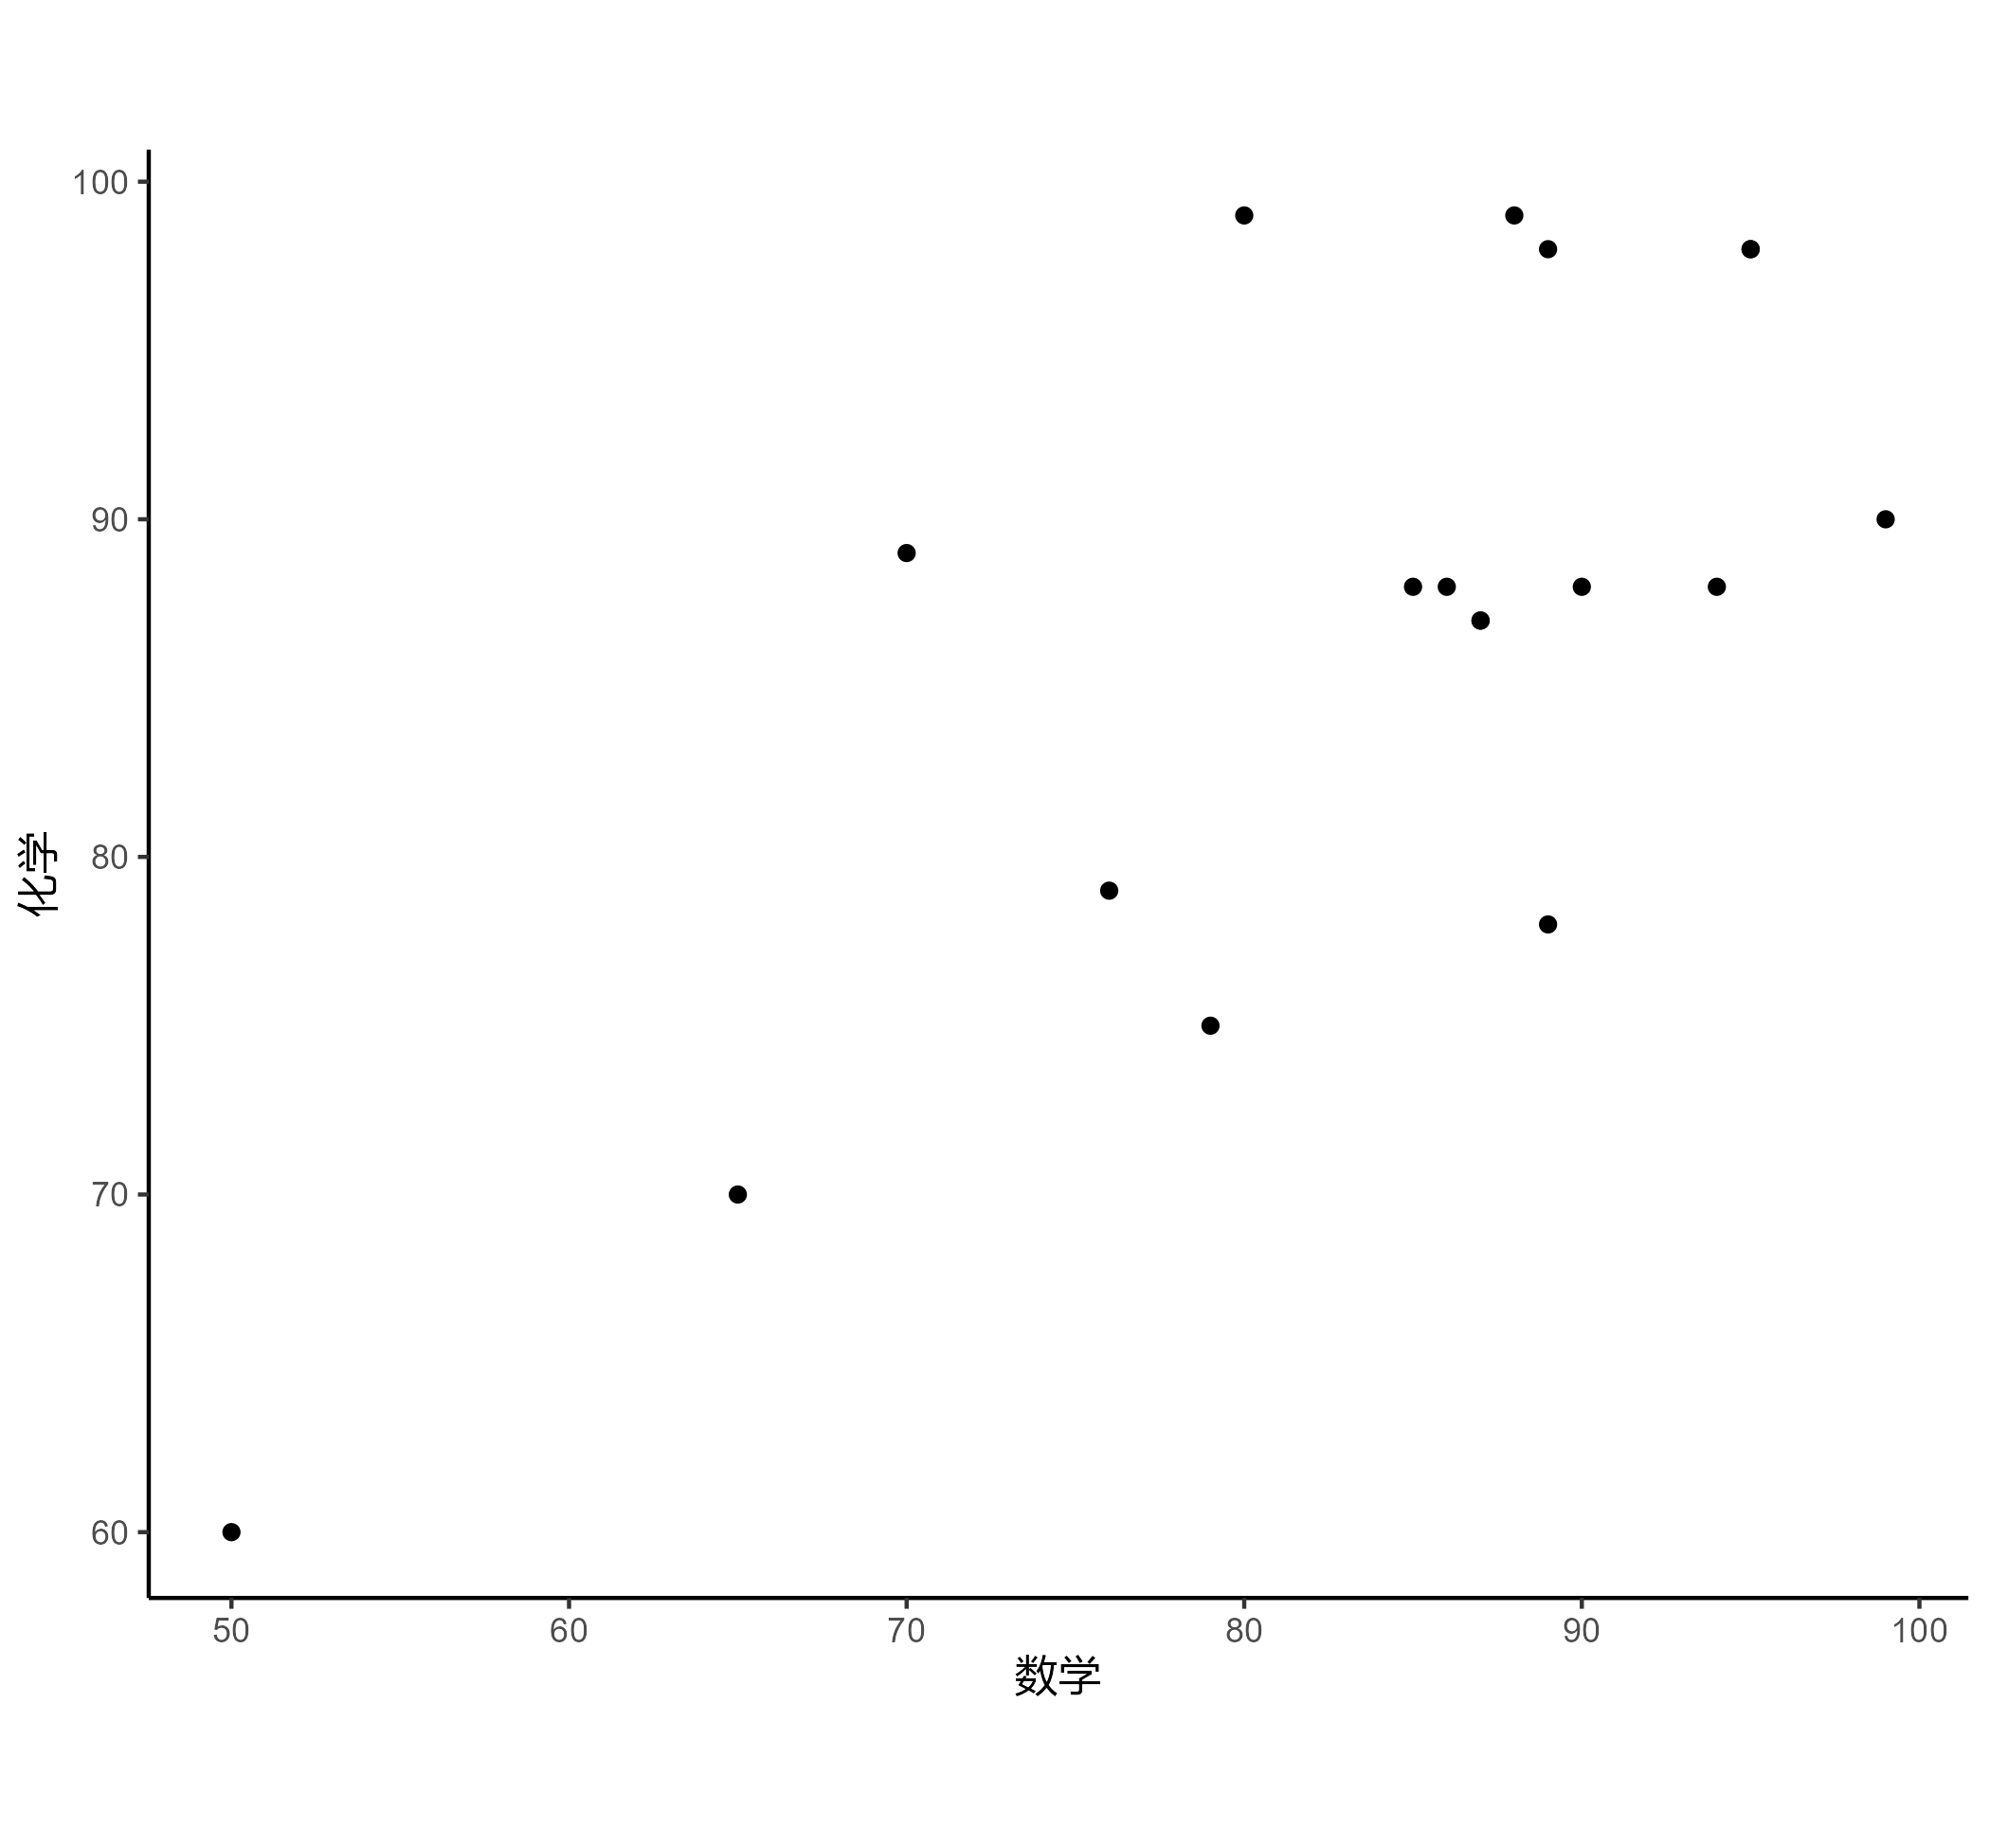
\includegraphics[width=1\linewidth,height=1\textheight]{exp2_files/figure-latex/cor1.png} \end{center}

\subsection{Spearman等级相关系数、Kendall's
等级相关系数计算}\label{spearmanux7b49ux7ea7ux76f8ux5173ux7cfbux6570kendalls-ux7b49ux7ea7ux76f8ux5173ux7cfbux6570ux8ba1ux7b97}

\begin{Shaded}
\begin{Highlighting}[]
\NormalTok{df\_rank }\OtherTok{=}\NormalTok{ readxl}\SpecialCharTok{::}\FunctionTok{read\_xls}\NormalTok{(}\StringTok{\textquotesingle{}../data/exp2/2.xls\textquotesingle{}}\NormalTok{,}\AttributeTok{sheet =} \StringTok{\textquotesingle{}Spearman\textquotesingle{}}\NormalTok{)}
\CommentTok{\# 计算Spearman等级相关系数}
\FunctionTok{cor.test}\NormalTok{(df\_rank}\SpecialCharTok{$}\StringTok{\textasciigrave{}}\AttributeTok{作文1}\StringTok{\textasciigrave{}}\NormalTok{,}
\NormalTok{         df\_rank}\SpecialCharTok{$}\StringTok{\textasciigrave{}}\AttributeTok{作文2}\StringTok{\textasciigrave{}}\NormalTok{,}
         \AttributeTok{method =} \StringTok{"spearman"}\NormalTok{)}
\end{Highlighting}
\end{Shaded}

\begin{verbatim}
## 
##  Spearman's rank correlation rho
## 
## data:  df_rank$作文1 and df_rank$作文2
## S = 122.56, p-value = 2.199e-06
## alternative hypothesis: true rho is not equal to 0
## sample estimates:
##       rho 
## 0.8735153
\end{verbatim}

\emph{作文1和作文2的\texttt{spearman}相关系数为\textbf{0.8735153},P值为\textbf{2.199e-06},两者在0.01显著性水平下相关性显著}

\begin{Shaded}
\begin{Highlighting}[]
\CommentTok{\# 计算Kendall\textquotesingle{}s等级相关系数}
\FunctionTok{cor.test}\NormalTok{(df\_rank}\SpecialCharTok{$}\StringTok{\textasciigrave{}}\AttributeTok{作文1}\StringTok{\textasciigrave{}}\NormalTok{,}
\NormalTok{         df\_rank}\SpecialCharTok{$}\StringTok{\textasciigrave{}}\AttributeTok{作文2}\StringTok{\textasciigrave{}}\NormalTok{,}
         \AttributeTok{method =} \StringTok{"kendall"}\NormalTok{)}
\end{Highlighting}
\end{Shaded}

\begin{verbatim}
## 
##  Kendall's rank correlation tau
## 
## data:  df_rank$作文1 and df_rank$作文2
## z = 4.2307, p-value = 2.33e-05
## alternative hypothesis: true tau is not equal to 0
## sample estimates:
##       tau 
## 0.7451175
\end{verbatim}

\emph{作文1和作文2的\texttt{kendall}相关系数为\textbf{0.7451175},P值为\textbf{2.33e-05},两者在0.01显著性水平下相关性显著}

\subsection{偏相关系数计算}\label{ux504fux76f8ux5173ux7cfbux6570ux8ba1ux7b97}

\begin{Shaded}
\begin{Highlighting}[]
\NormalTok{df\_p }\OtherTok{=}\NormalTok{ readxl}\SpecialCharTok{::}\FunctionTok{read\_xls}\NormalTok{(}\StringTok{\textquotesingle{}../data/exp2/2.xls\textquotesingle{}}\NormalTok{,}\AttributeTok{sheet =} \StringTok{\textquotesingle{}偏相关\textquotesingle{}}\NormalTok{)}
\CommentTok{\# 控制变量为温度}
\NormalTok{ppcor}\SpecialCharTok{::}\FunctionTok{pcor.test}\NormalTok{(}\AttributeTok{x =}\NormalTok{ df\_p}\SpecialCharTok{$}\NormalTok{产量,}
                 \AttributeTok{y =}\NormalTok{ df\_p}\SpecialCharTok{$}\NormalTok{降雨量,}
                 \AttributeTok{z =}\NormalTok{ df\_p}\SpecialCharTok{$}\NormalTok{温度)}
\end{Highlighting}
\end{Shaded}

\begin{verbatim}
##    estimate    p.value statistic  n gp  Method
## 1 0.7802799 0.01310611  3.300809 10  1 pearson
\end{verbatim}

\emph{当控制变量为温度时,产量和降雨量的偏相关系数为\textbf{0.7802799},且P值\textbf{0.01310611}小于0.05,说明产量和降雨量相关性显著.}

\begin{Shaded}
\begin{Highlighting}[]
\CommentTok{\# 控制变量为降雨量}
\NormalTok{ppcor}\SpecialCharTok{::}\FunctionTok{pcor.test}\NormalTok{(}\AttributeTok{x =}\NormalTok{ df\_p}\SpecialCharTok{$}\NormalTok{产量,}
                 \AttributeTok{y =}\NormalTok{ df\_p}\SpecialCharTok{$}\NormalTok{温度,}
                 \AttributeTok{z =}\NormalTok{ df\_p}\SpecialCharTok{$}\NormalTok{降雨量)}
\end{Highlighting}
\end{Shaded}

\begin{verbatim}
##    estimate    p.value statistic  n gp  Method
## 1 0.8462227 0.00402605  4.201899 10  1 pearson
\end{verbatim}

\emph{当控制变量为降雨量时,产量和温度的偏相关系数为\textbf{0.8462227},且P值\textbf{0.00402605}小于0.05,说明产量和温度相关性显著.}

\end{document}
